In this section we study the interaction of a so called "coronal hole" with an MHD wave as introduced in the paper \cite{coronal-hole} by A.N. Afanasyev and A. N. Zhukov. 
A coronal hole is a region in the coronal with much lower density and a lower temperature than the surrounding area.
A the coronal hole was simulated in 2.5d, assuming that the variables do not depend on $z$ but the $z$-components of vectors do not need to be zero.
An ideal equation of state is assumed, this gives the following relation between density, temperature and pressure:
\begin{equation}
	nk_BT = p
	\label{eq:ideal-gas}
\end{equation}
The total pressure $p^T$ is given by [REF], from there the magnitude of the magnetic field is calculated as follows (expressions for code units):
\begin{equation}
	B = \sqrt{2 \left( p^T-p \right) }
	\label{eq:magnetic-magnitude}
\end{equation}
The total pressure inside and outside the coronal hole is kept in equilibrium by changing the magnitude of the magnetic field accordingly.

\subsection{Initial and boundary conditions}

The parameters for the coronal hole are the same as in \cite{coronal-hole}. 
The physical size of the domain is a square with sidelength $2\times 10^{11}cm$, the grid used for the simulation has $1024$ by $1024$ gridpoints. As a model for the number density and temperature the following was used:
\begin{equation}
	\label{eq:hole-model}
	\begin{split}
		n(r) &= n_{out} - (n_{out}-n_{in})\exp \left( -(r/d)^8 \right)\\
		T(r) &= T_{out} - (T_{out}-T_{in})\exp \left( -(r/d)^8 \right) 
	\end{split}
\end{equation}
$r$ represents the distance from the center of the hole and $d$ the characteristic size of the hole. 
The parameters $n_{out}, n_{in}, T_{out}$ and $T_{in}$ are respectively the plasma number density outside and inside the hole, the temperature outside and the temperature inside the hole. 
The magnetic field has zero $x$ and $y$ component and the $z$ component is calculated according to \cref{eq:magnetic-magnitude}.
The total pressure is calculated by fixing a value $B_{out}$ for the magnitude of the magnetic field far away from the hole, and calculated using [ref].
As a counterpart to the coronal hole model a coronal plume model was considered as well, again based on \cite{coronal-hole}.
Here the density outside the plume is a lot lower than the density inside.
The parameter values for both models can be found in \cref{tab:parameters-hole}.
In \cref{fig:hole-initial} and \cref{fig:plume-initial} the value of some impotant quantities at $t=0$ are shown along a section through the center of the hole or plume respectively.

\begin{table}[H]
	\centering
	\begin{tabular}{|l|r|r|}
		\toprule
		Parameter & Coronal hole & Coronal plume\\
		\midrule
		$n_{out}$ & $1.0\times 10^9$ cm$^{-3}$ & $1.0\times 10^8$ cm$^{-3}$\\
		$n_{in}$ & $1.0\times 10^8$ cm$^{-3}$ & $1.0\times 10^9$ cm$^{-3}$\\
		$T_{out}$ & $1.5\times 10^6$ K & $1.5\times 10^6$ K\\
		$T_{in}$ & $1.0\times10^6$ K & $1.0\times10^6$ K\\
		$d$ & $1.5\times10^{10}$ m& $1.0\times10^{10}$ m \\
		$B_{out} $ & $4.0$ G & $3.0$ G\\
		\midrule
		$v_m$ & $50$ km s$^{-1}$ & $125$ km s$^{-1}$ \\
		$s_1$ & $20$ s & $60$ s \\
		$s_2$ & $16$ s& $50$ s\\
		\bottomrule
	\end{tabular}
	\caption{Parameter values taken from \cite{coronal-hole}. The values used for the initial condition of the coronal hole and coronal plume models.}
	\label{tab:parameters-hole}
\end{table}
For the nonlinear wave driver the velocity along $x$ was perturbed at the left boundaryi. 
To smoothly transition from $0$ to a certain max velocity $v_m$, stay at this velocity for some time and smoothly go back to $0$ a combination of two hyperbolic tangents is used in the following formula:
\begin{equation}
	v_x(t) = v_m \tanh \left( \frac{t}{s_1} \right) - \frac{v_m}{2} \left( \tanh \left( \frac{t-T_0}{s_2} \right) +1 \right) 
\end{equation}
The parameters $s_1$ and $s_2$ control the steepnes of the transition from $v=0$ to $v=v_m$.
$T_0$ controls the time when the velocity drops back from $v_m$ to $0$, at $t=0$ the velocity starts increasing immediatly.
This wave propagates with the speed of a fast magnetoaccoustic wave transverse to the magnetic field (in the $z$-direction).
Using \cref{eq:magnetoaccoustic-group-speed} we find that the group speed of the fast magnetoacoustic wave transverse to the magnetic field is:
\begin{equation*}
	v_{g+} = \sqrt{v_a^2+v_s^2}
\end{equation*}
From \cref{fig:hole-initial} and \cref{fig:plume-initial} it is clear that this speed is a lot higher outside the plume than outside the hole (about $2.5$ times).
To get a wave of the same physical width in both simulations, we use a shorter wave pulse in the coronal plume model with slightly steeper edges and higher maximum velocity.
The parameters for the waves can again be found in \cref{tab:parameters-hole}.

At the right boundary an open boundary condition is used. For the top and bottom boundaries a periodic boundary condition is used.

\begin{figure}[H]
	%\hspace{-1cm}
	\centering
	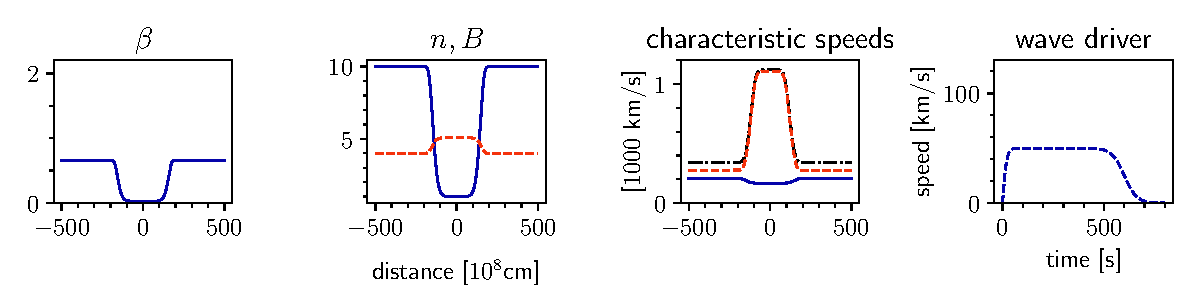
\includegraphics[width=.9\linewidth]{images/sections-initial-condition-hole.pdf}
	\caption{Sections of the initial condition for the \emph{coronal hole} model. 
		\emph{First plot}: plasma beta as given by [REF], dimensionless quantity.
		\emph{Second plot}: the full blue line is the plasma number density in $10^8$ cm$^{-3}$.
The red dashed line is the magentic field in Gauss.
\emph{Third plo}t: full line is the sound speed $v_s$, dashed red line the Alfvén speed $v_a$ and the dash-dotted black line the fast magnetoaccoustic speed $v_+$.
\emph{Last plo}t: speed profile of the wave driver used.
Adapted from \cite{coronal-hole}}
	\label{fig:hole-initial}
\end{figure}

\begin{figure}[H]
	%\hspace{-1cm}
	\centering
	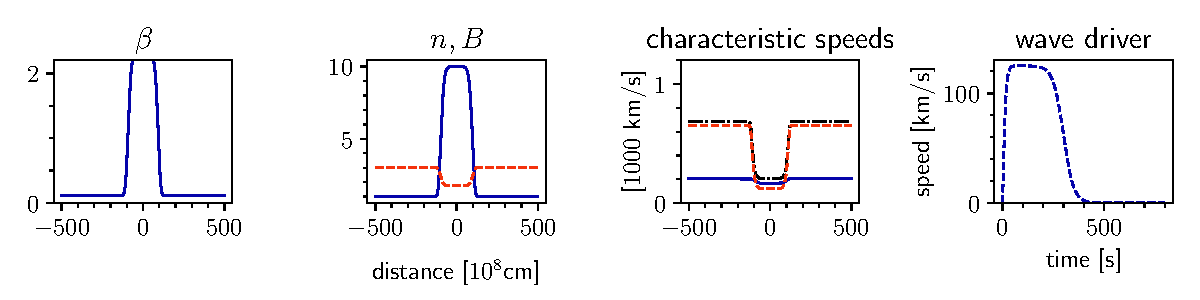
\includegraphics[width=.9\linewidth]{images/sections-initial-condition-plume.pdf}
	\caption{Same as \cref{fig:hole-initial} but for the \emph{coronal plum}e model.}
	\label{fig:plume-initial}
\end{figure}

\todo{Add a clearer discussion about terminology used}
\subsection{Terminolgy}
Before we dive into the discussion of our simulation results, first some comments on the terminology used.
Our discussion is mainly based on \cref{fig:hole-frames}, \cref{fig:plume-frames}, \cref{fig:hole-sections} and \cref{fig:plume-sections}.

\Cref{fig:hole-frames} and \cref{fig:plume-frames} contain snapshots at 6 different timestamps.
For each timestamps, two plots are made next to each other.
One plot contains heatmap of the complete simulation domain representing the density, next to it is again a density heatmap, this time zoomed in on the whit box in the plot next to it, providing a better view of the hole/plume.
The limits for the colormap are chosen in such a way to highlight the wavefronts, the units of the labels are $10^9$particles cm$^{-3}$.
When we reference a frame, we talk about the two plots with the same timestamp. If we talk about behaviour inside the hole/plume, this about the right plot of the pair.
Behaviour outside the structure is about the left plot of the pair.

\Cref{fig:hole-sections} and \cref{fig:plume-sections} contain plots of the density along a cut through the center of the hole or plume along the direction of propagation of the wave.
The top and middle plot show the wave outside the structure, the bottom plot zooms in on the wave inside the structure.
The dashed lines show the position of the waveforont at the bottom edge of the simulation domain.

We will often talk about the transmitted and reflected waves, as well as the "main" wave. 
The transmitted wave is the wave that travels through the structure when it comes back out of the structure.
This is for instance the red ring right of the hole in the fourth frame in \cref{fig:hole-frames} and the red ring around the plume in the last frame of \cref{fig:plume-frames}.
The reflected wave denotes the wave comming from the left, top and bottom of the hole/plume right after the main wave comes in contact with the structure.
The main wave is the wave generated at the left boundary.


\subsection{Results coronal hole}
In \cref{fig:hole-frames} a couple of density profiles of the \emph{coronal hole} simulation are plotted.
From \cref{fig:hole-initial} we see that the speed of the wave (the fast magnetoaccoustic speed) is a lot hihger inside than outside the hole.
Therefore it is expected that the wave transmitted through the hole will be faster then the wave going around.
This effect is visible in the heatmaps in \cref{fig:hole-frames}. 
In the image at $t=2.97e+3s$ the wave fron of the transmitted wave is barely vissible, a siginficant amount before the main wavefront.
The frames at later times show that the main wave slowly cathche up with the transmitted wave. This is probably due to non-linear effects in the shock-wave.

This fast transmission is most clearly seen in \cref{fig:hole-sections}. 
At $t=2.5e+3 s$ the wave is almost at the center of the hole, while the wavefront at the edge of the simulation domain (the green dashed line) is already lagging $100\times10^{11} cm$ behind.
Comparing with the snapshot at $t=2.55e+3$ shows that the wavefront inside the hole, which has traveled about $50\times10^{11}$ cm since the previous snapshot travels about $2.5$ times faster than the wav outside the hole, covering only $20\times10^{11}$ cm in the same timespan.
We also remark that the effect of the wave on the hole is to suddenly increase the density, this is the wavefront seen in the snapshots previously discussed.
When the wave passed, the density drops back to it's original value, but the position where it reaches it's lowest value is shifted along the direction of propagation of the wave.

Two other phenomena that are readily observed in the last three frames are the diffraction of the main wave around the hole and a rarefraction wave reflected from the hole.
At $t=2.97e+3$ and $t=3.42e+03$ we see the wave bending around the hole, and interfering with the transmitted wave.
In the last frame the deffracted wave is vissible behind the transmitted wavefront, both slightly less energetic than the main wave.
The incomming wave also reflects from the hole.
In the fourth frame a black region just behind the hole is visible, this is the reflected rarefraction wave (wave with lower density, in contrast to a shock wave with higher density) closely followed by a wavefron with slightly higher density.
We see that the reflected wave has oposite phase compared to the incomming wave.
Because this wave is almost perfectly circular with the same radius as the transmitted wave, measured from the center of the hole, it is clear this wave travels at the fast magnetoaccoustic speed as well.

These two effects alter the density of the plasma, the transmitted wava has a lower density compared to the main wave, but higher than the surrounding plasma and the rarefraction wave has a lower density than the surrounding.
Therefore, by altering the density they alter the brightness of the plasma. 
If the hole itself is not directly observable local dimming of a wave, together with a dimmer wave traveling backwards, can point to a local sudden decrease in density.
Furthermore, by carefully studying the form of these waves and amount of dimming it might be possible to extract more information about the parameters of the non-uniformity such as size and relative change in density.

Lastly, we note that the holes position is slightly shifted along de direction of propagation of the wave.
Apart from a slight deformation of the center of the hole where the density is almost uniform, its shape stays largely unaltered.

\begin{figure}[H]
	%\hspace{-1cm}
	\centering
	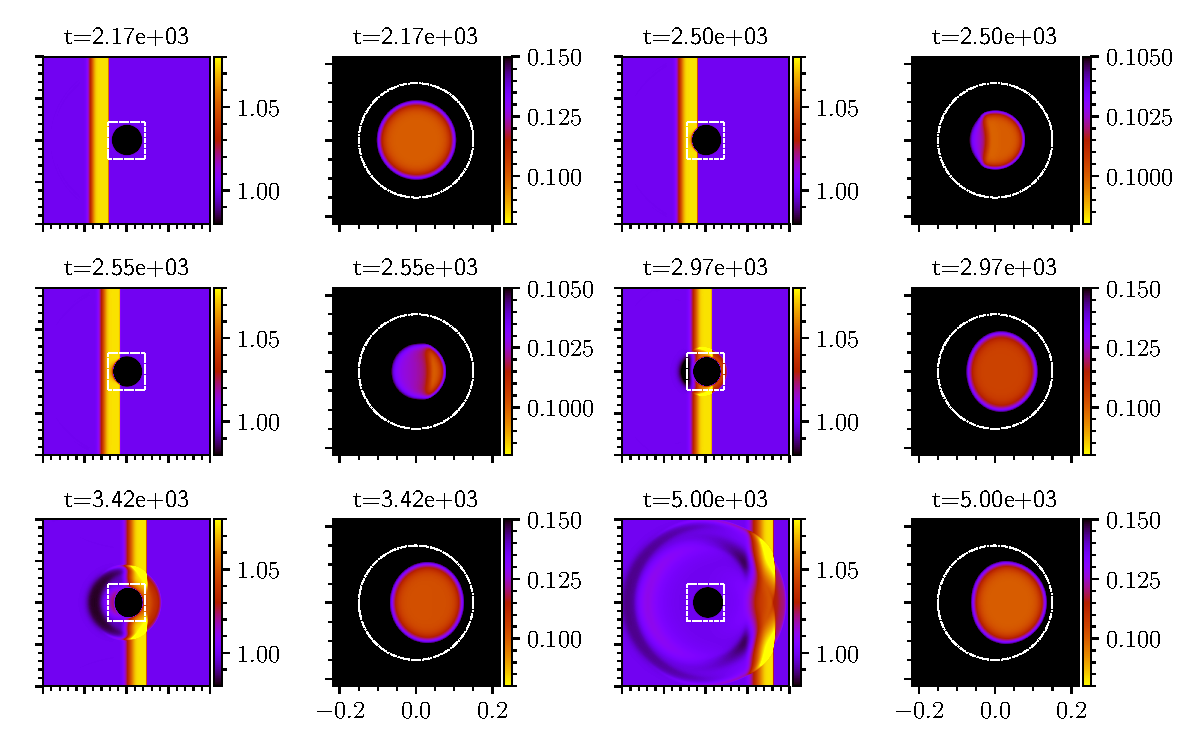
\includegraphics[width=\linewidth]{images/hole-frames.pdf}
	\caption{Plots of the density profile of the \emph{coronal hole model} for different times. 
	The plots in the first and third column cover de complete domain.
	The plots in the second and last column are zooms on the plume. 
	The domain covered is the white box in the plots to the left.
 The density is measured in $10^{9}$ cm$^{-3}$.
The white circle has the characteristic width $d$ as diameter. 
In the second an third pair of plots, the density range for the right plot is taken a lot more narrow to highlight the wave transmitted through the coronal hole.}
	\label{fig:hole-frames}
\end{figure}

\begin{figure}[H]
	%\hspace{-1cm}
	\centering
	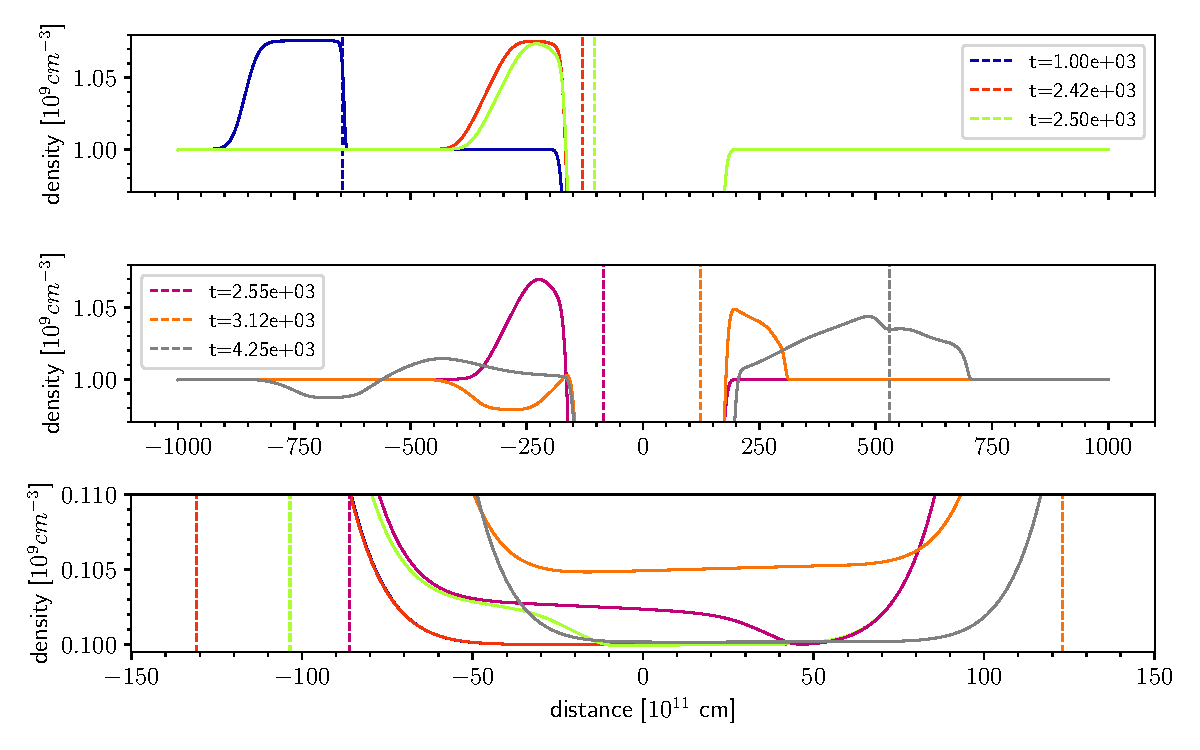
\includegraphics[width=\linewidth]{images/hole-sections.pdf}
	\caption{Density profiles along a cut, parallel to the direction of propagation of the wave, through the center of the \emph{coronal hole} at different times. The vertical dashed lines show the position of the wavefront at the bottom edge of the simulation domain.}
	\label{fig:hole-sections}
\end{figure}


\begin{figure}[H]
	%\hspace{-1cm}
	\centering
	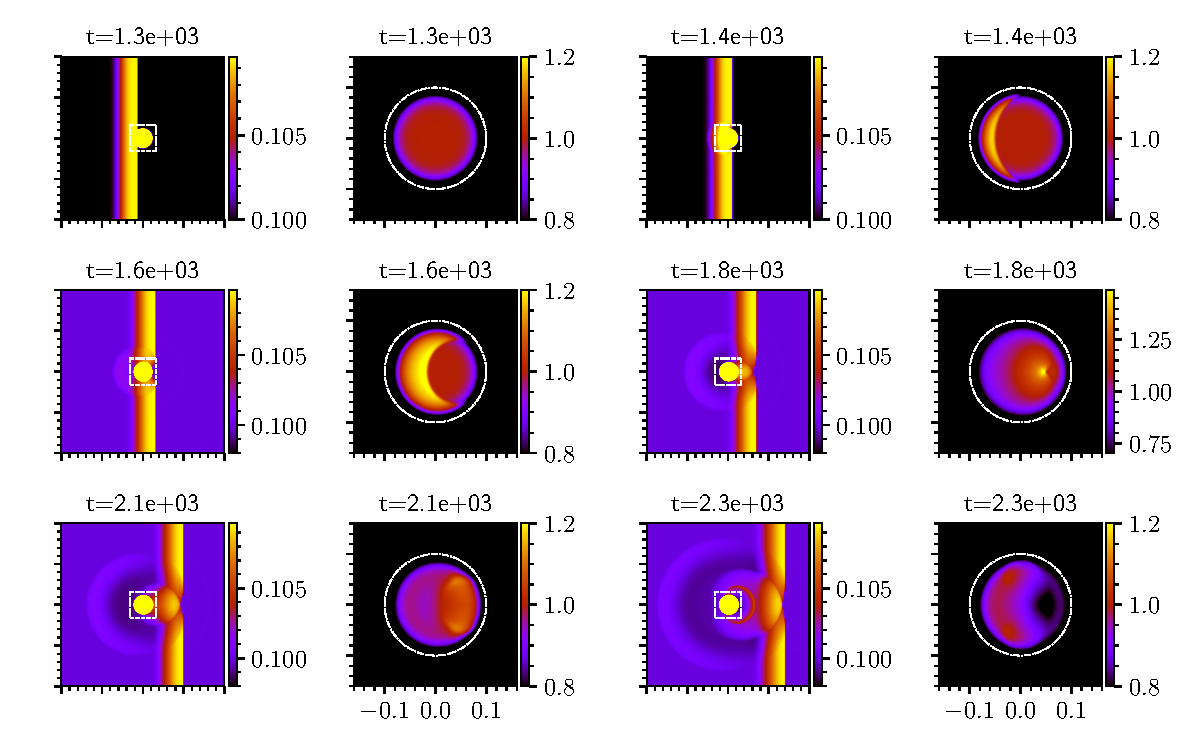
\includegraphics[width=\linewidth]{images/plume-frames.pdf}
	\caption{Plots of density profiles for the \emph{coronal plume model}. Same conventions used as in \cref{fig:hole-frames}}
	\label{fig:plume-frames}
\end{figure}

\begin{figure}[H]
	%\hspace{-1cm}
	\centering
	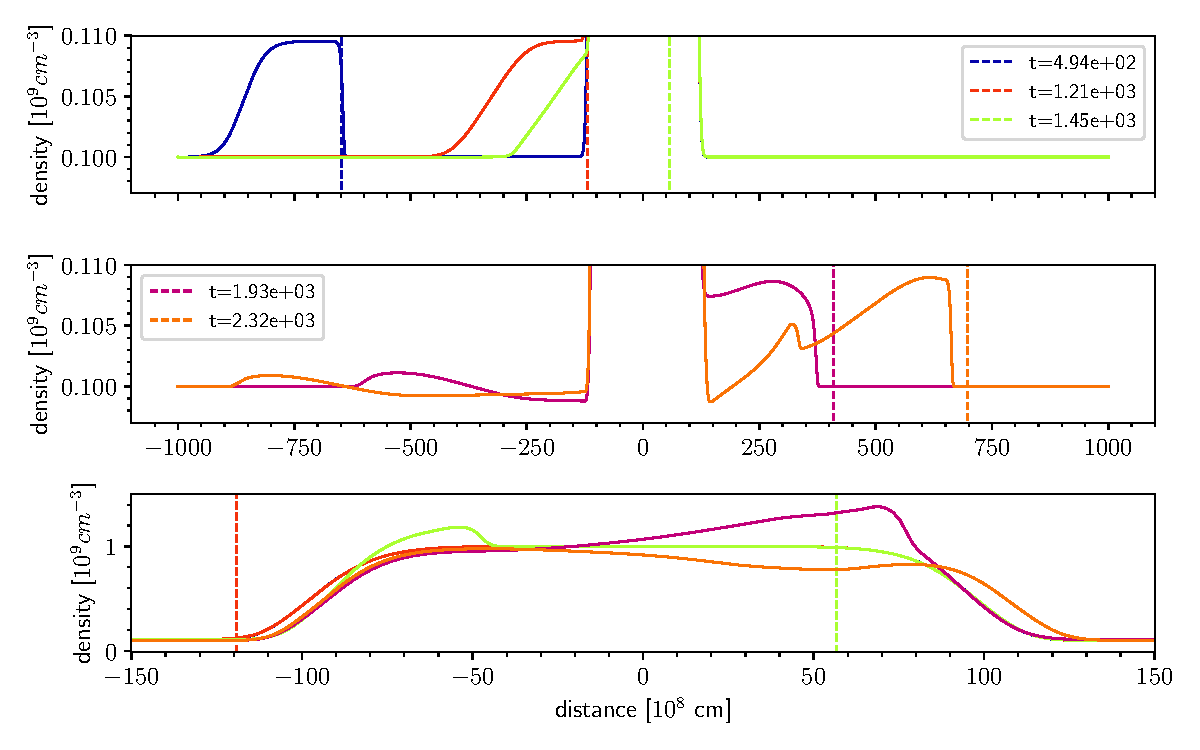
\includegraphics[width=\linewidth]{images/plume-sections.pdf}
	\caption{Density profiles along a cut through the center of the \emph{coronal plume} at different times, along the direction of propagation of the waves.
	The vertical dashed lines show the position of the wave at the bottom edge of the simulation domain.}
	\label{fig:plume-sections}
\end{figure}

\subsection{Results coronal plume}

Next we discuss the \emph{coronal plume model}. There is again a refelcted wave visible.
In \cref{fig:plume-sections} we see that now there is a wavefront with slightly higher density first, followed by a lower density wake by looking at the snapshots for $t=1.93e+3 s$ and $t=2.32e+3 s$.
We see that the the wave reflected when going from fast to slow magnetoaccoustic speed is in phase, while the reflected wave going from low to high magnetoaccoustic speed is out of phase.
This second fact was already observed in the case of the coronal hole, but can also be seen in the zoomed in images of the plume or the density profiles along a cut in the plume.
Between the frames at $t=2.1e+3 s$ and $t=2.3+e3$ in \cref{fig:plume-frames}  or $t=1.93e+3 s$ and $t=2.32e+3 s$ in \cref{fig:plume-sections} the wave inside the plume reflects at the boundary and switches from a significantly higher density than the surroundig area to lower density, therefore switching phase.

In this case the transmitted wave is, as expected, slower than the wave outside the hole.
this is clearly visible as the line corresponding to $t=2.32e+3 s$ in the second plot of \cref{fig:plume-sections}.
The original wavefront is clearly visible with in its wake a small spike, this is the transmitted wave.
Furthermore, the wave get's captured inside the plume which functions as an echo chamber emitting secondary wavefronts.
Such a secondary wave can be seen as the red ring forming in the last frame in $\cref{fig:plume-frames}$.

In the plume the formation of a caustic is observed in the fourth frame of \cref{fig:plume-frames}. 
The density increase caused by the wave is focussed in almost a single point here. 
This is due to the wave refracting when entering the hole which makes the plume function like a lens and a slight deformation will probably lead to less striking caustics.
In fact, there were also caustics in the coronal hole model.
In the frames at the bottom in figure \cref{fig:hole-frames} we see bright edges where the reflected/transmitted wave meets the main wave.

We see again that the structure is moved slightly along the direction of propagation of the wave. 
If there is a deformation of the coronal plume, it is a lot smaller than in the case of the coronal hole model.

Just as in the coronal hole model the wave is deformed by the interaction with the structure.
The transmitted wave forms a second wave front behind the main wavefront, which is deformed by diffraction around the hole.













